\documentclass[]{article}
\usepackage{lmodern}
\usepackage{amssymb,amsmath}
\usepackage{ifxetex,ifluatex}
\usepackage{fixltx2e} % provides \textsubscript
\ifnum 0\ifxetex 1\fi\ifluatex 1\fi=0 % if pdftex
  \usepackage[T1]{fontenc}
  \usepackage[utf8]{inputenc}
\else % if luatex or xelatex
  \ifxetex
    \usepackage{mathspec}
  \else
    \usepackage{fontspec}
  \fi
  \defaultfontfeatures{Ligatures=TeX,Scale=MatchLowercase}
\fi
% use upquote if available, for straight quotes in verbatim environments
\IfFileExists{upquote.sty}{\usepackage{upquote}}{}
% use microtype if available
\IfFileExists{microtype.sty}{%
\usepackage{microtype}
\UseMicrotypeSet[protrusion]{basicmath} % disable protrusion for tt fonts
}{}
\usepackage[margin=1in]{geometry}
\usepackage{hyperref}
\hypersetup{unicode=true,
            pdftitle={Market Basket Analysis Report},
            pdfauthor={Ivan Sokolenko, Alejo Gonzalez Mata, Joan Figueras},
            pdfborder={0 0 0},
            breaklinks=true}
\urlstyle{same}  % don't use monospace font for urls
\usepackage{graphicx,grffile}
\makeatletter
\def\maxwidth{\ifdim\Gin@nat@width>\linewidth\linewidth\else\Gin@nat@width\fi}
\def\maxheight{\ifdim\Gin@nat@height>\textheight\textheight\else\Gin@nat@height\fi}
\makeatother
% Scale images if necessary, so that they will not overflow the page
% margins by default, and it is still possible to overwrite the defaults
% using explicit options in \includegraphics[width, height, ...]{}
\setkeys{Gin}{width=\maxwidth,height=\maxheight,keepaspectratio}
\IfFileExists{parskip.sty}{%
\usepackage{parskip}
}{% else
\setlength{\parindent}{0pt}
\setlength{\parskip}{6pt plus 2pt minus 1pt}
}
\setlength{\emergencystretch}{3em}  % prevent overfull lines
\providecommand{\tightlist}{%
  \setlength{\itemsep}{0pt}\setlength{\parskip}{0pt}}
\setcounter{secnumdepth}{0}
% Redefines (sub)paragraphs to behave more like sections
\ifx\paragraph\undefined\else
\let\oldparagraph\paragraph
\renewcommand{\paragraph}[1]{\oldparagraph{#1}\mbox{}}
\fi
\ifx\subparagraph\undefined\else
\let\oldsubparagraph\subparagraph
\renewcommand{\subparagraph}[1]{\oldsubparagraph{#1}\mbox{}}
\fi

%%% Use protect on footnotes to avoid problems with footnotes in titles
\let\rmarkdownfootnote\footnote%
\def\footnote{\protect\rmarkdownfootnote}

%%% Change title format to be more compact
\usepackage{titling}

% Create subtitle command for use in maketitle
\providecommand{\subtitle}[1]{
  \posttitle{
    \begin{center}\large#1\end{center}
    }
}

\setlength{\droptitle}{-2em}

  \title{Market Basket Analysis Report}
    \pretitle{\vspace{\droptitle}\centering\huge}
  \posttitle{\par}
    \author{Ivan Sokolenko, Alejo Gonzalez Mata, Joan Figueras}
    \preauthor{\centering\large\emph}
  \postauthor{\par}
      \predate{\centering\large\emph}
  \postdate{\par}
    \date{12/04/2019}


\begin{document}
\maketitle

{
\setcounter{tocdepth}{4}
\tableofcontents
}
\subsection{Executive summary:}\label{executive-summary}

\begin{center}\rule{0.5\linewidth}{\linethickness}\end{center}

\subsection{Introduction:}\label{introduction}

To gather all the neccessery insights about Electroindex's business
activity, we have used their online transactions data and a file
containing all the electronics that they currently sell. Due to their
lack of funding, Electronidex is only able to pull data on the items
that customers purchased per their transactions, meaning that we cannot
identify whether the same customer made multiple transactions during
this time period.

\subsection{Insights and findings:}\label{insights-and-findings}

Using insights from previous analysis of Blackwell's products, we can
see that products that have the highest volume sold are accessories and
displays, which have shown to have a strong association with desktops
and laptops in the Electroindex's data set.

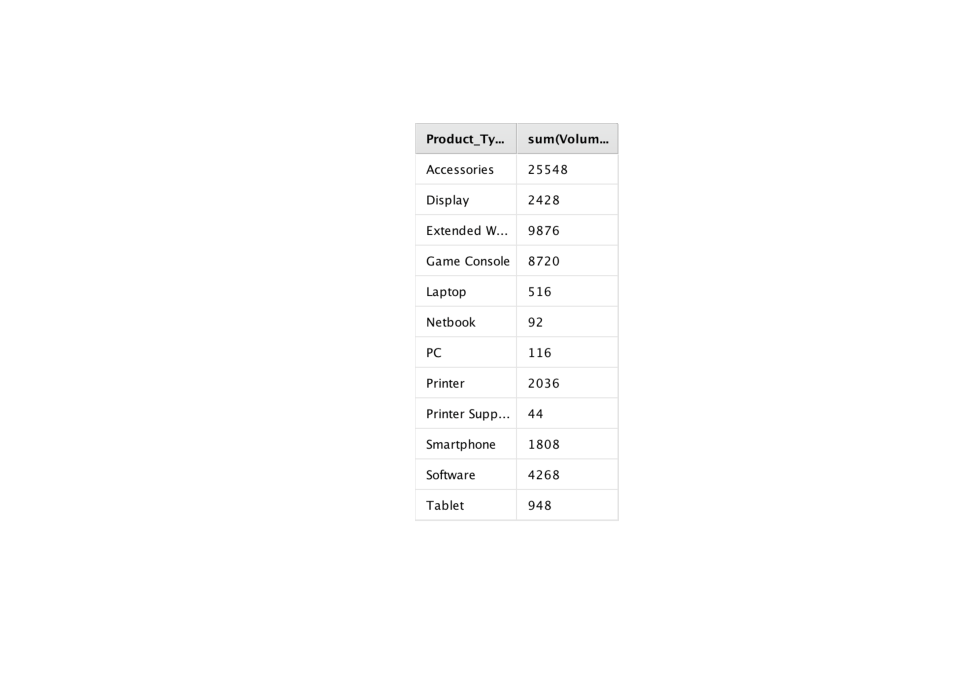
\includegraphics{markdown_report_files/figure-latex/pic1-1.pdf}

We also know that products that have the highest predicted profitability
for Blackwell are Tablets and PCs, shown on the ranked table below:

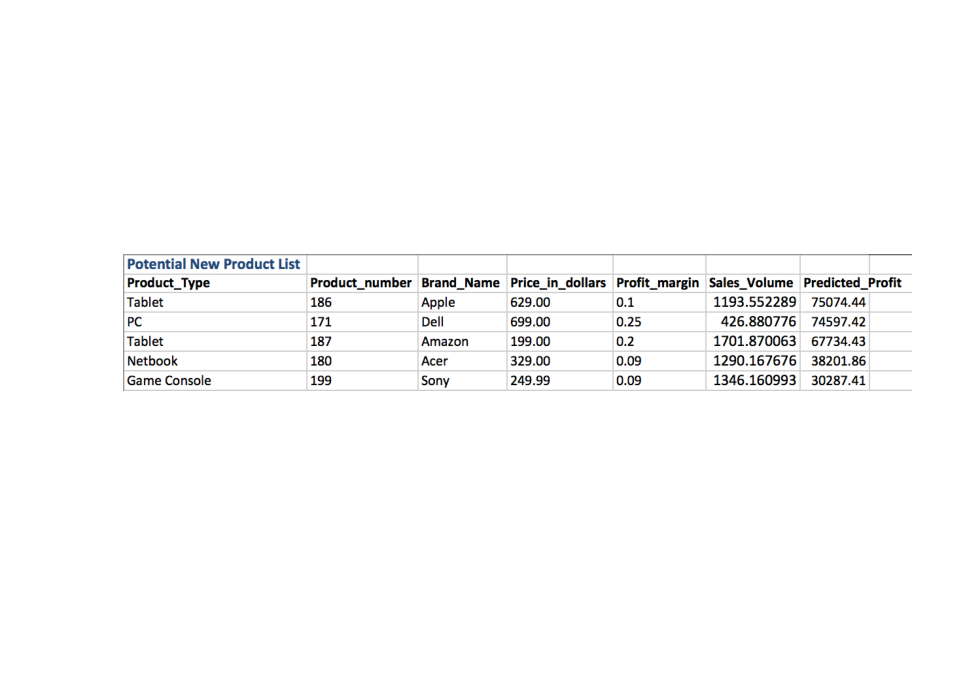
\includegraphics{markdown_report_files/figure-latex/pic2-1.pdf}

Using product association insights and the above information, we can
conclude that Blackwell can gain profits in the following way if it
decides to buy Electroindex:

\begin{enumerate}
\def\labelenumi{\arabic{enumi})}
\item
  Since PCs have the most predicted profit for Blackwell and
  Electroindex's most sold items are PCs, it should use Electroindex's
  products such as PCs/Desktops/Laptops as it's product supply and
  bundle them with already existing Blackwell's accessories.
\item
  Because there is a strong association between accessories and PCs,
  everytime a customer buys a PC, using targeted marketing Blackwell
  could offer bundles or suggestions for customers to also buy
  accessories, which in most cases will provide extra profit.
\end{enumerate}

\begin{verbatim}
## Number of transactions
## [1] 9835
##      items                                                                                               
## [1]  Acer Aspire + Belkin Mouse Pad + Brother Printer Toner + VGA Monitor Cable                          
## [2]  Apple Wireless Keyboard + Dell Desktop + Lenovo Desktop Computer                                    
## [3]  iMac                                                                                                
## [4]  Acer Desktop + Intel Desktop + Lenovo Desktop Computer + XIBERIA Gaming Headset                     
## [5]  ASUS Desktop + Epson Black Ink + HP Laptop + iMac                                                   
## [6]  ASUS Monitor + Gaming Mouse Professional + iMac + Lenovo Desktop Computer + Mackie CR Speakers      
## [7]  CYBERPOWER Gamer Desktop                                                                            
## [8]  Apple MacBook Air + Bose Companion Speakers + CYBERPOWER Gamer Desktop + HP Laptop + Large Mouse Pad
## [9]  Logitech Keyboard                                                                                   
## [10] Generic Black 3-Button + iMac
## Number of transactions per item: /n
## [1] "1 Item --> 2163"
## [1] "2 Item --> 1647"
## [1] "3 Item --> 1294"
## [1] "4 Item --> 1021"
## [1] "5 Item --> 856"
## [1] "6 Item --> 646"
\end{verbatim}

While doing market basket analysis, we have discovered some strong
associations between Electroindex's products. In particular, a lot of
customers who shop at Electroindex will purchase ``bundles'' of
products, mainly as a combination of desktop/laptop and accessories. We
have also found out that Electroindex's most sold products are desktops
and laptops, which you can see on the graph below:

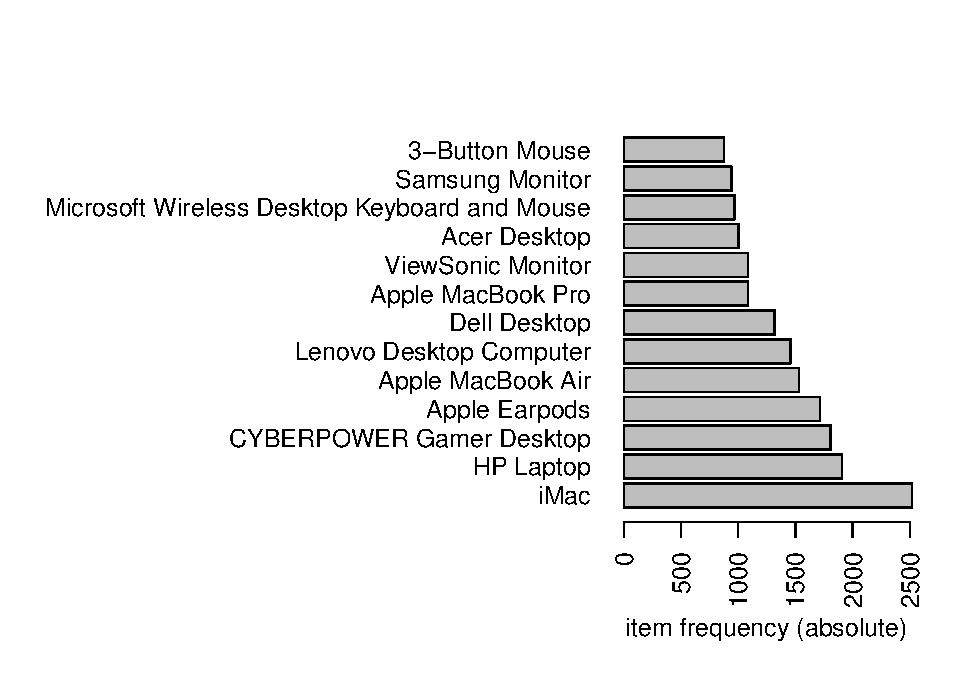
\includegraphics{markdown_report_files/figure-latex/Plots By Items-1.pdf}

\begin{verbatim}
## 
## Rules Sorted by lift 
##      lhs                                                                                     
## [1]  Dell KM117 Wireless Keyboard & Mouse + iPhone Charger Cable                             
## [2]  HP Monitor + iMac + Koss Home Headphones                                                
## [3]  3-Button Mouse + Acer Desktop + ASUS Monitor                                            
## [4]  Acer Aspire + Dell Desktop + iMac + ViewSonic Monitor                                   
## [5]  Epson Printer + iMac + Lenovo Desktop Computer + ViewSonic Monitor                      
## [6]  Dell Desktop + HP Monitor + Lenovo Desktop Computer + ViewSonic Monitor                 
## [7]  Etekcity Power Extension Cord Cable + iMac + Lenovo Desktop Computer + ViewSonic Monitor
## [8]  3-Button Mouse + Acer Aspire + ViewSonic Monitor                                        
## [9]  Apple Magic Keyboard + Epson Printer + iMac + Lenovo Desktop Computer                   
## [10] Computer Game + Dell Desktop + ViewSonic Monitor                                        
##         rhs                     support     confidence lift     count
## [1]  => Apple MacBook Air       0.002033554 0.9523810  6.122004 20   
## [2]  => Lenovo Desktop Computer 0.001525165 0.8823529  5.960124 15   
## [3]  => HP Laptop               0.001525165 0.9375000  4.829917 15   
## [4]  => HP Laptop               0.003762074 0.9024390  4.649286 37   
## [5]  => HP Laptop               0.001728521 0.8947368  4.609605 17   
## [6]  => HP Laptop               0.001728521 0.8947368  4.609605 17   
## [7]  => HP Laptop               0.001626843 0.8888889  4.579477 16   
## [8]  => HP Laptop               0.001525165 0.8823529  4.545805 15   
## [9]  => HP Laptop               0.001525165 0.8823529  4.545805 15   
## [10] => HP Laptop               0.002643620 0.8666667  4.464990 26   
## 
## Rules Sorted by support 
##      lhs                                                                         
## [1]  Acer Aspire + Dell Desktop + ViewSonic Monitor                              
## [2]  Acer Aspire + Dell Desktop + iMac + ViewSonic Monitor                       
## [3]  Acer Desktop + Dell Desktop + iMac + ViewSonic Monitor                      
## [4]  Dell Desktop + Mackie CR Speakers                                           
## [5]  Computer Game + Dell Desktop + ViewSonic Monitor                            
## [6]  Dell Desktop + HP Black & Tri-color Ink                                     
## [7]  CYBERPOWER Gamer Desktop + HP Black & Tri-color Ink                         
## [8]  ASUS 2 Monitor + ASUS Monitor + Lenovo Desktop Computer                     
## [9]  ASUS 2 Monitor + Dell Desktop + Microsoft Office Home and Student 2016      
## [10] Apple Magic Keyboard + Dell Desktop + Microsoft Office Home and Student 2016
##         rhs       support     confidence lift     count
## [1]  => HP Laptop 0.005287239 0.8125000  4.185928 52   
## [2]  => HP Laptop 0.003762074 0.9024390  4.649286 37   
## [3]  => HP Laptop 0.003253686 0.8000000  4.121530 32   
## [4]  => iMac      0.002643620 0.8666667  3.383750 26   
## [5]  => HP Laptop 0.002643620 0.8666667  4.464990 26   
## [6]  => iMac      0.002541942 0.8064516  3.148651 25   
## [7]  => iMac      0.002440264 0.8000000  3.123462 24   
## [8]  => iMac      0.002440264 0.8000000  3.123462 24   
## [9]  => iMac      0.002440264 0.8275862  3.231167 24   
## [10] => iMac      0.002440264 0.8275862  3.231167 24   
## 
## Rules Sorted by confidence 
##      lhs                                                                                             
## [1]  Apple Magic Keyboard + Rii LED Gaming Keyboard & Mouse Combo + ViewSonic Monitor                
## [2]  Etekcity Power Extension Cord Cable + HP Laptop + Lenovo Desktop Computer + ViewSonic Monitor   
## [3]  Dell KM117 Wireless Keyboard & Mouse + iPhone Charger Cable                                     
## [4]  Dell Desktop + Lenovo Desktop Computer + Samsung Monitor + ViewSonic Monitor                    
## [5]  ASUS 2 Monitor + Dell Desktop + Lenovo Desktop Computer + Microsoft Office Home and Student 2016
## [6]  ASUS Desktop + Dell Desktop + iPad Pro                                                          
## [7]  3-Button Mouse + Acer Desktop + ASUS Monitor                                                    
## [8]  ASUS Monitor + Dell Desktop + Lenovo Desktop Computer + ViewSonic Monitor                       
## [9]  Acer Aspire + Dell Desktop + iMac + ViewSonic Monitor                                           
## [10] Epson Printer + iMac + Lenovo Desktop Computer + ViewSonic Monitor                              
##         rhs               support     confidence lift     count
## [1]  => iMac              0.001728521 1.0000000  3.904327 17   
## [2]  => iMac              0.001626843 1.0000000  3.904327 16   
## [3]  => Apple MacBook Air 0.002033554 0.9523810  6.122004 20   
## [4]  => iMac              0.001830198 0.9473684  3.698836 18   
## [5]  => iMac              0.001728521 0.9444444  3.687420 17   
## [6]  => iMac              0.001525165 0.9375000  3.660307 15   
## [7]  => HP Laptop         0.001525165 0.9375000  4.829917 15   
## [8]  => iMac              0.001931876 0.9047619  3.532486 19   
## [9]  => HP Laptop         0.003762074 0.9024390  4.649286 37   
## [10] => HP Laptop         0.001728521 0.8947368  4.609605 17
\end{verbatim}


\end{document}
